% ==============================================================
% 08_final_presentation.tex
% "Money and Success in Football: Does Financial Strength
%  Predict League Position?"
% Beamer / Metropolis — compile with pdflatex (TWICE)
% ==============================================================
\documentclass[aspectratio=169,10pt]{beamer}

% ── Metropolis theme ──────────────────────────────────────────
\usetheme[progressbar=frametitle, block=fill]{metropolis}

% ── pdflatex font & encoding compatibility ───────────────────
\usepackage[T1]{fontenc}
\usepackage{lmodern}
\usepackage{textcomp}   % \texteuro, \textsterling, \textrightarrow
\usepackage{microtype}

% ── Core packages ─────────────────────────────────────────────
\usepackage{graphicx}
\usepackage{booktabs}
\usepackage{colortbl}
\usepackage{xcolor}
\usepackage{tikz}
\usepackage{array}
\usepackage{amsmath}
\usepackage{url}
\usepackage{calc}

% ── Image path ────────────────────────────────────────────────
\graphicspath{{outputs/}}

% ── Project colour palette ────────────────────────────────────
\definecolor{NavyBlue}{HTML}{1A2A4A}
\definecolor{PitchGold}{HTML}{F5A623}
\definecolor{AlertRed}{HTML}{C0392B}
\definecolor{GrassGreen}{HTML}{196F3D}
\definecolor{SteelBlue}{HTML}{2C3E73}
\definecolor{SlateGrey}{HTML}{566573}
\definecolor{RowA}{HTML}{EBF5FB}
\definecolor{RowB}{HTML}{FEF9E7}

% ── Metropolis colour overrides ───────────────────────────────
\setbeamercolor{normal text}{fg=NavyBlue, bg=white}
\setbeamercolor{frametitle}{bg=NavyBlue, fg=white}
\setbeamercolor{title separator}{fg=PitchGold}
\setbeamercolor{progress bar}{fg=PitchGold, bg=NavyBlue!25}
\setbeamercolor{progress bar in section page}{fg=PitchGold, bg=NavyBlue!25}
\setbeamercolor{alerted text}{fg=AlertRed}
\setbeamercolor{example text}{fg=GrassGreen}
\setbeamercolor{block title}{bg=NavyBlue!12, fg=NavyBlue}
\setbeamercolor{block body}{bg=NavyBlue!5, fg=NavyBlue}
\setbeamercolor{block title alerted}{bg=AlertRed!12, fg=AlertRed}
\setbeamercolor{block body alerted}{bg=AlertRed!5}
\setbeamercolor{block title example}{bg=GrassGreen!12, fg=GrassGreen}
\setbeamercolor{block body example}{bg=GrassGreen!5}

\metroset{titleformat=smallcaps}

% ── Presentation metadata ─────────────────────────────────────
\title{Money and Success in Football}
\subtitle{Does Financial Strength Predict League Position?}
\author{Md.~Muktadir}
\date{Summer Semester 2026}
\institute{Sports Economics Seminar}

% ── tikzpicture-based callout boxes (preamble) ────────────────
% Gold-bordered key finding box
\newcommand{\findingbox}[1]{%
  \begin{tikzpicture}
    \node[
      fill        = PitchGold!18,
      draw        = PitchGold,
      line width  = 0.9pt,
      rounded corners = 4pt,
      inner sep   = 10pt,
      text width  = \linewidth-10pt
    ]{\small\bfseries\color{NavyBlue}#1};
  \end{tikzpicture}%
}

% Red-bordered alert box
\newcommand{\alertbox}[1]{%
  \begin{tikzpicture}
    \node[
      fill        = AlertRed!10,
      draw        = AlertRed,
      line width  = 0.9pt,
      rounded corners = 4pt,
      inner sep   = 10pt,
      text width  = \linewidth-10pt
    ]{\small\bfseries\color{AlertRed}#1};
  \end{tikzpicture}%
}

% Stat panel: big number + small caption
\newcommand{\statpanel}[2]{%
  \begin{tikzpicture}
    \node[
      fill        = NavyBlue!7,
      draw        = NavyBlue!25,
      line width  = 0.6pt,
      rounded corners = 4pt,
      inner sep   = 10pt,
      text width  = \linewidth-10pt,
      align       = center
    ]{%
      {\large\bfseries\color{NavyBlue}#1}%
      \par\smallskip
      {\footnotesize\color{SlateGrey}#2}%
    };
  \end{tikzpicture}%
}

% Dual-language annotation (statistician label / plain English label)
\newcommand{\duallabel}[2]{%
  \begin{tikzpicture}
    \node[
      fill        = RowA,
      draw        = SteelBlue!30,
      line width  = 0.5pt,
      rounded corners = 3pt,
      inner sep   = 8pt,
      text width  = \linewidth-10pt
    ]{%
      {\footnotesize\textbf{\color{SteelBlue}Statistical view:} #1}%
      \par\smallskip
      {\footnotesize\textbf{\color{GrassGreen}Plain English:} #2}%
    };
  \end{tikzpicture}%
}

% ─────────────────────────────────────────────────────────────
\begin{document}

\maketitle

% ──────────────────────────────────────────────────────────────
%  SECTION 1: Introduction
% ──────────────────────────────────────────────────────────────
\section{Introduction}

\begin{frame}{The Billion-Euro Question}
  \begin{columns}[T]
    \begin{column}{0.54\textwidth}
      \vspace{4pt}
      \begin{itemize}
        \setlength\itemsep{8pt}
        \item The five major European leagues spent over
              \textbf{\color{AlertRed}\texteuro{}12 billion}
              on transfers in 2023\textendash{}24 alone.
        \item Fan debate: does buying expensive squads
              actually \emph{buy} titles?
        \item Or can a \textbf{well-organised, under\-funded club}
              still win?
      \end{itemize}
      \vspace{10pt}
      \findingbox{This study uses 10 years of data from
        5 leagues (975 team-seasons) to answer with evidence,
        not opinion.}
    \end{column}
    \begin{column}{0.42\textwidth}
      \vspace{4pt}
      \begin{block}{Three Research Questions}
        \begin{enumerate}
          \setlength\itemsep{6pt}
          \item Does financial rank predict league position?
          \item \emph{How much} of the variation does
                money explain?
          \item Who defies the financial logic entirely?
        \end{enumerate}
      \end{block}
    \end{column}
  \end{columns}
\end{frame}

% ──────────────────────────────────────────────────────────────
%  SECTION 2: Data & Methodology
% ──────────────────────────────────────────────────────────────
\section{Data \& Methodology}

\begin{frame}{Five Leagues, Ten Seasons \textendash{} 975 Observations}
  \begin{columns}[T]
    \begin{column}{0.50\textwidth}
      \vspace{2pt}
      {\small
      \begin{tabular}{%
          >{\bfseries}l r r r}
        \toprule
        \rowcolor{NavyBlue!18}
        \color{white}\textbf{League} &
        \color{white}\textbf{N} &
        \color{white}\textbf{Seasons} &
        \color{white}\textbf{$r$(FR,Pos)} \\
        \midrule
        Bundesliga     & 180 & 10 & 0.783 \\
        \rowcolor{RowA}
        La Liga        & 200 & 10 & 0.787 \\
        Ligue~1        & 196 & 10 & 0.791 \\
        \rowcolor{RowA}
        Premier League & 200 & 10 & 0.801 \\
        Serie~A        & 199 & 10 & 0.889 \\
        \midrule
        \rowcolor{RowB}
        \textbf{All} & \textbf{975} & \textbf{10} & \textbf{0.813} \\
        \bottomrule
      \end{tabular}
      }
      \vspace{6pt}
      {\footnotesize\color{SlateGrey}
        Seasons: 2015\textendash{}16 to 2024\textendash{}25.
        All $r$ values significant at $p < 0.001$.}
    \end{column}
    \begin{column}{0.46\textwidth}
      \vspace{2pt}
      \begin{block}{Key Variable: Financial Rank (FR)}
        \begin{itemize}
          \setlength\itemsep{5pt}
          \item Squads ranked by squad market value
                \textbf{within each league-season}.
          \item \textbf{FR = 1} = richest squad that season.\\
                \textbf{FR = 20} = least wealthy.
          \item Normalising within leagues removes
                between-league scale differences
                (Premier League values $\approx3\times$
                Bundesliga).
        \end{itemize}
      \end{block}
      \vspace{4pt}
      \duallabel{%
        Spearman $\rho = 0.814$, Pearson $r = 0.813$;
        both $p < 0.001$.}{%
        The wealth ranking of a squad is an almost
        perfect mirror of its final position.}
    \end{column}
  \end{columns}
\end{frame}

% ──────────────────────────────────────────────────────────────
%  SECTION 3: Statistical Evidence
% ──────────────────────────────────────────────────────────────
\section{Statistical Evidence}

\begin{frame}{Richer Squads Finish Higher \textendash{} Always}
  \begin{columns}[T]
    \begin{column}{0.64\textwidth}
      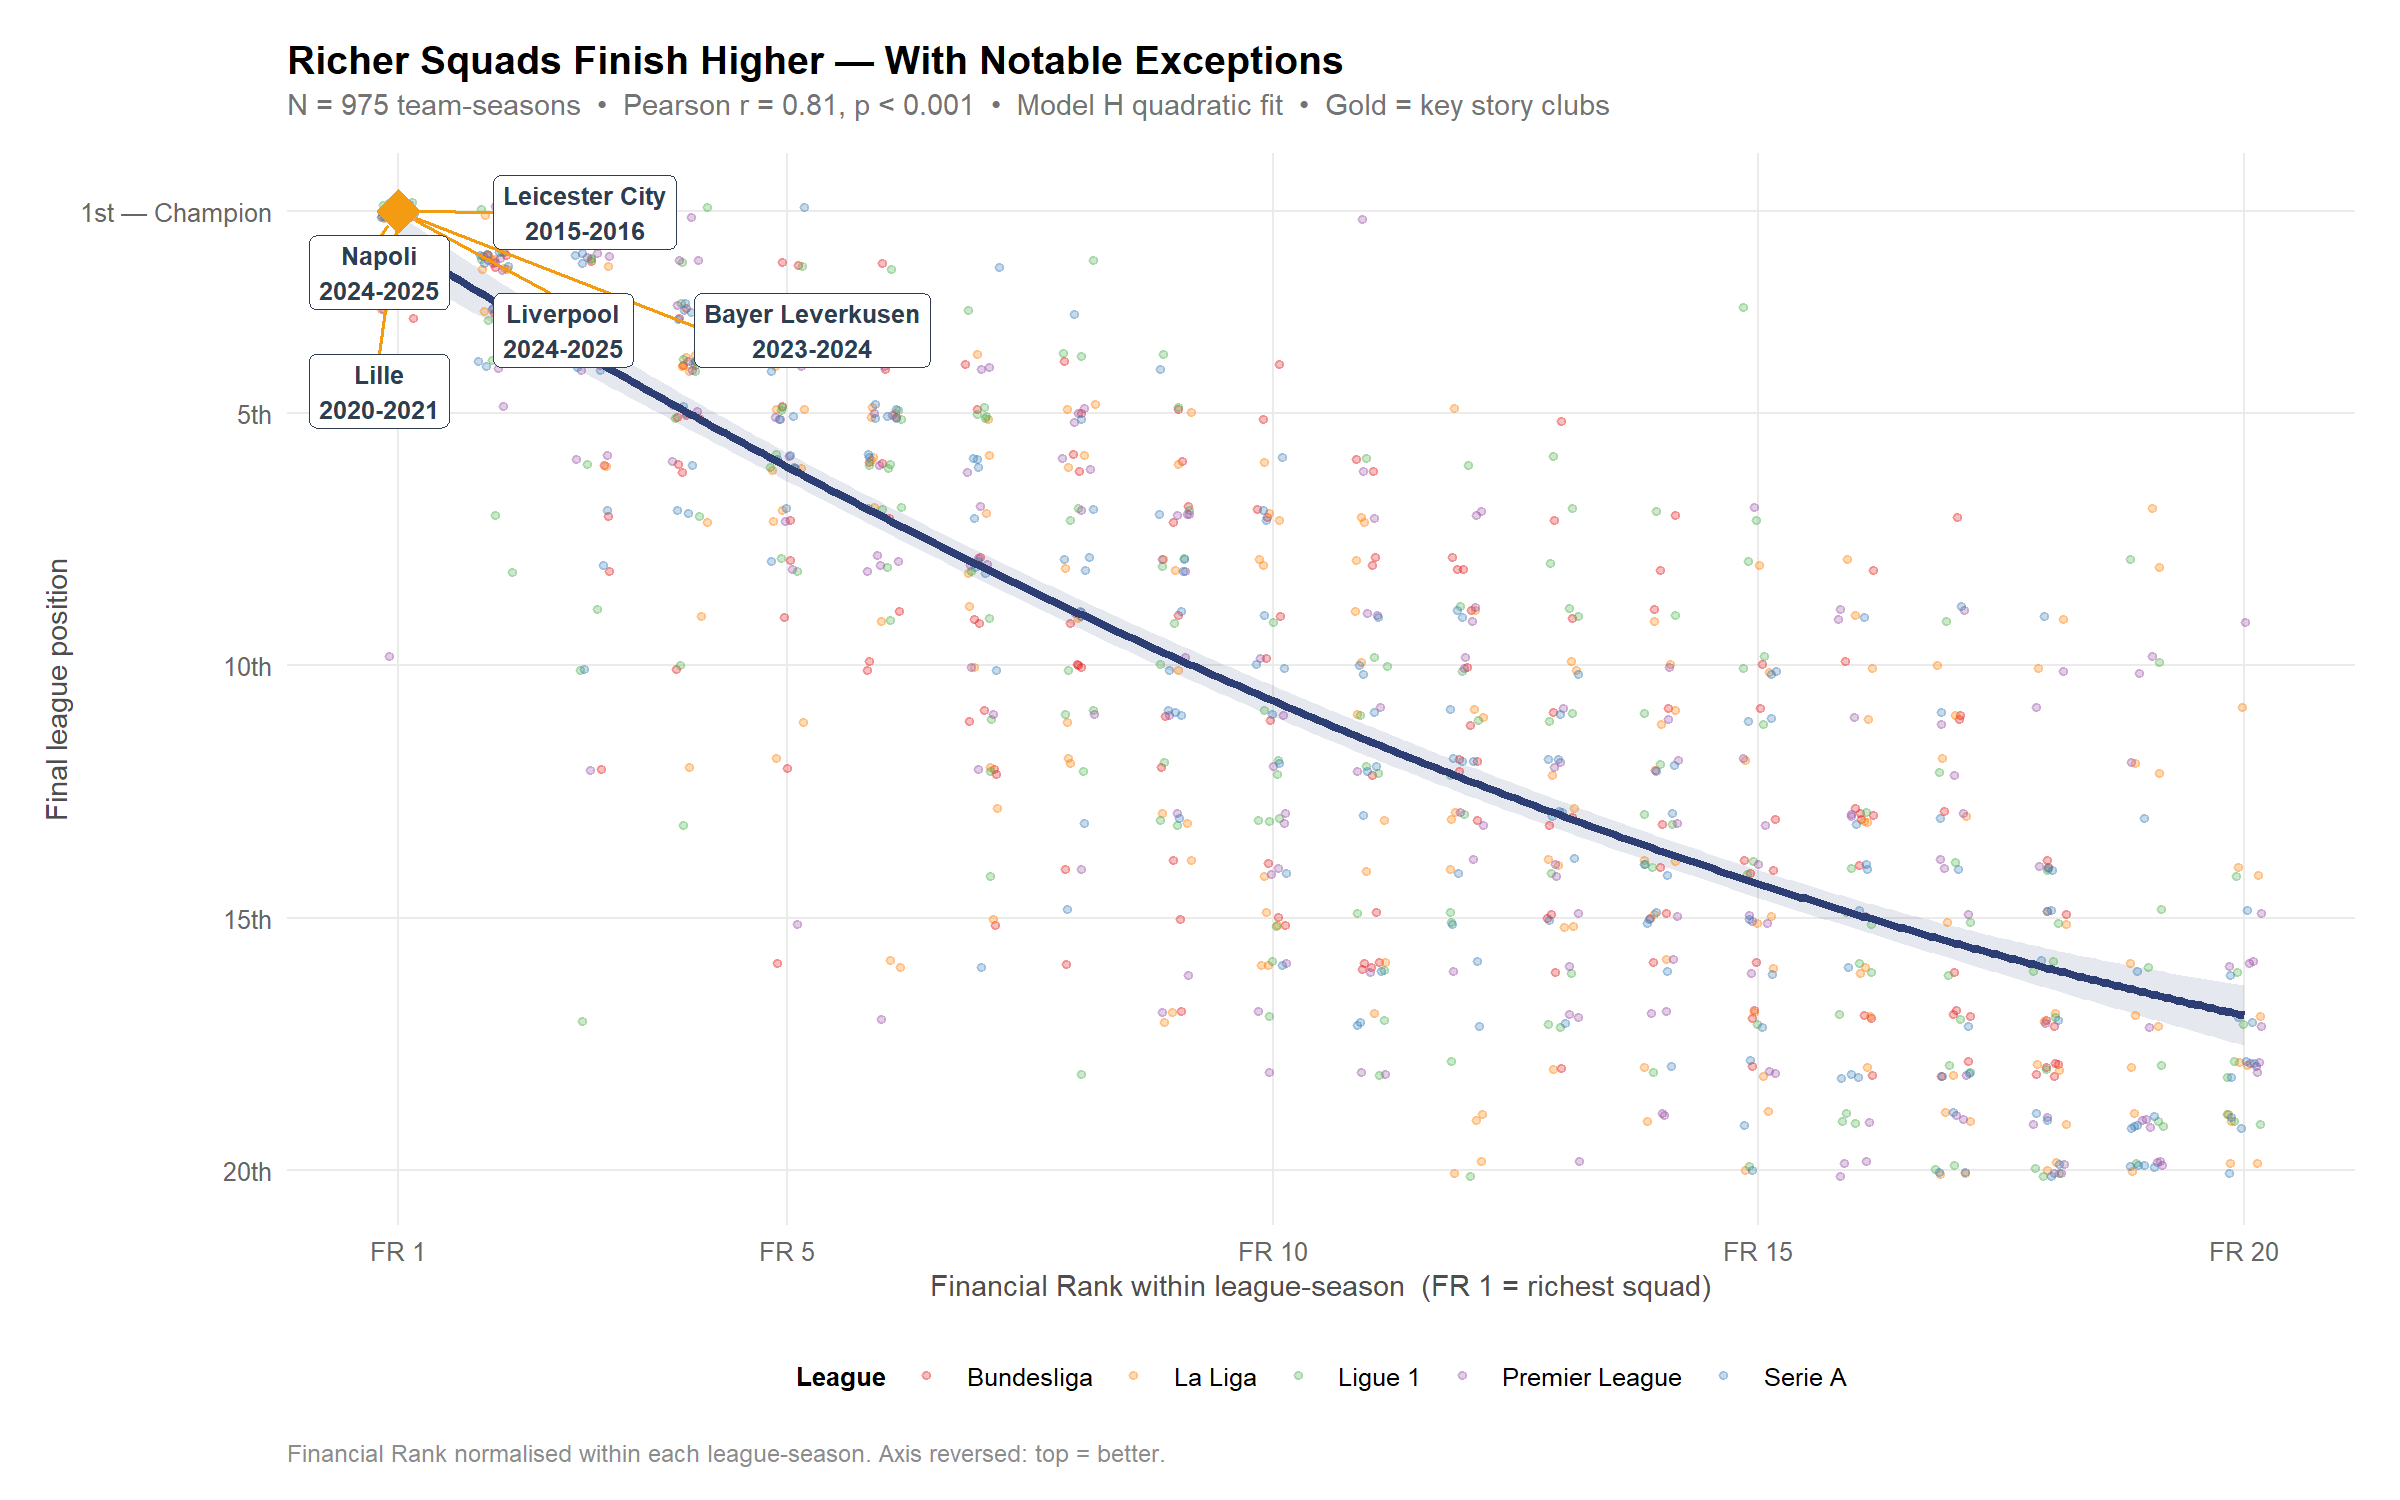
\includegraphics[width=\linewidth,
                       height=0.74\textheight,
                       keepaspectratio]{33_scatter_story.png}
    \end{column}
    \begin{column}{0.33\textwidth}
      \vspace{8pt}
      \statpanel{$r = 0.813$}{Pearson correlation,
        Financial Rank vs.\ Final Position\\
        $N=975$, $p<0.001$}
      \vspace{8pt}
      \begin{itemize}
        \setlength\itemsep{6pt}
        {\small
        \item \textbf{Gold diamonds} = five notable
              clubs whose finish surprised the model.
        \item Every league, every season: the
              upward trend holds.
        \item \alert{Exceptions exist}\,--- and they
              tell the real story.
        }
      \end{itemize}
    \end{column}
  \end{columns}
\end{frame}

\begin{frame}{The Effect Holds in Every League}
  \begin{columns}[T]
    \begin{column}{0.60\textwidth}
      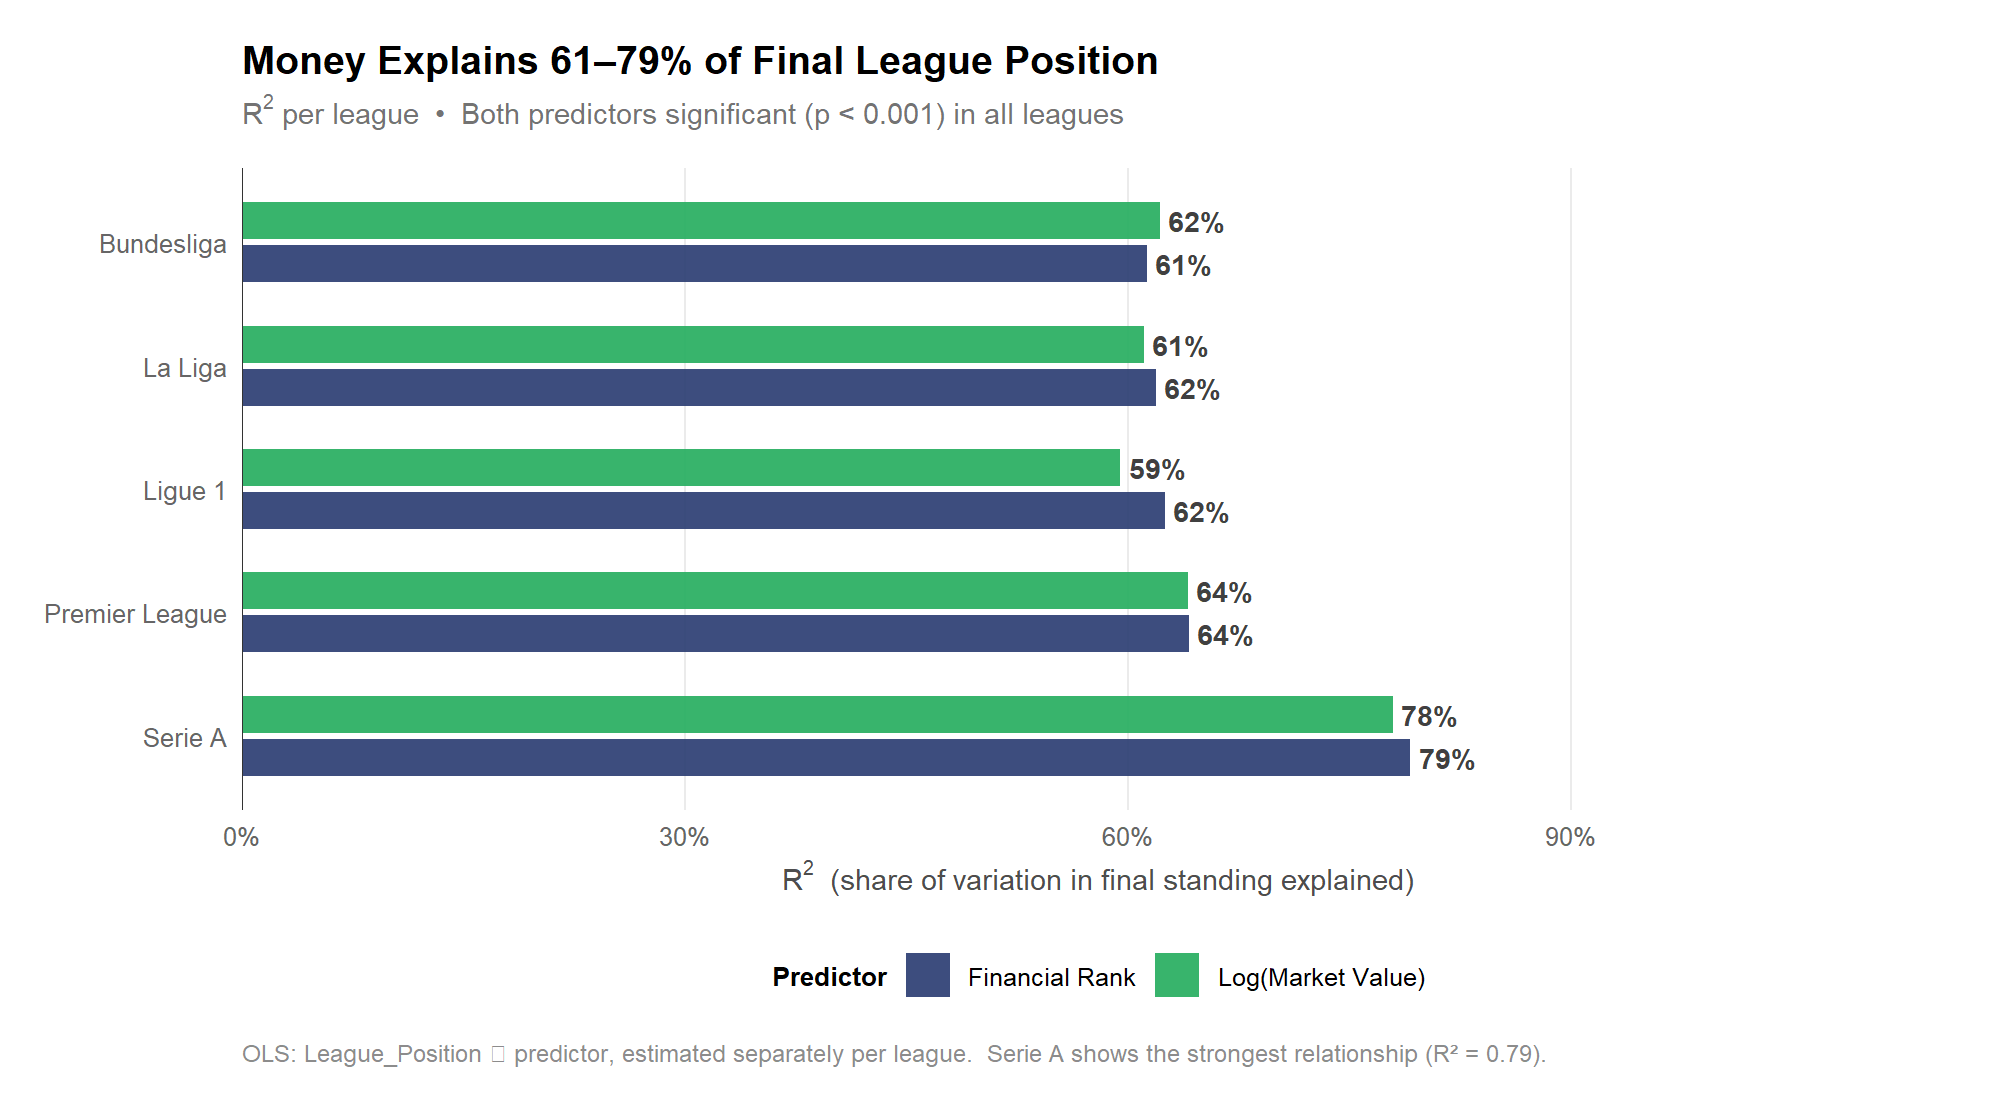
\includegraphics[width=\linewidth,
                       height=0.74\textheight,
                       keepaspectratio]{32_league_r2_bars.png}
    \end{column}
    \begin{column}{0.36\textwidth}
      \vspace{8pt}
      {\small
      \begin{tabular}{@{}l r@{}}
        \toprule
        \rowcolor{NavyBlue!18}
        \color{white}\textbf{League} &
        \color{white}\textbf{$R^2$} \\
        \midrule
        Bundesliga     & 0.613 \\
        \rowcolor{RowA}
        La Liga        & 0.619 \\
        Ligue~1        & 0.625 \\
        \rowcolor{RowA}
        Premier League & 0.641 \\
        \rowcolor{RowB}
        \textbf{Serie A} & \textbf{0.791} \\
        \bottomrule
      \end{tabular}
      }
      \vspace{8pt}
      \findingbox{Financial Rank alone explains
        61\textendash{}79\,\% of where a club
        finishes. In Serie~A the figure rises
        to 79\,\%.}
    \end{column}
  \end{columns}
\end{frame}

% ──────────────────────────────────────────────────────────────
%  SECTION 4: Model Results
% ──────────────────────────────────────────────────────────────
\section{Model Results}

\begin{frame}{Model H: The Best-Fitting Specification}
  \begin{columns}[T]
    \begin{column}{0.50\textwidth}
      \vspace{4pt}
      {\small
      \begingroup\setlength{\tabcolsep}{4pt}
      \begin{tabular}{@{}c p{4.5cm} c c@{}}
        \toprule
        \rowcolor{NavyBlue!18}
        \color{white}\textbf{Mdl} &
        \color{white}\textbf{Formula} &
        \color{white}\textbf{$R^2$} &
        \color{white}\textbf{AIC} \\
        \midrule
        A & FR only           & 0.660 & 5099.8 \\
        \rowcolor{RowA}
        B & FR + League FE    & 0.660 & 5107.4 \\
        C & Log(MV) only      & 0.533 & 5410.6 \\
        \rowcolor{RowA}
        D & Log(MV) + League + Season & 0.641 & 5164.3 \\
        \rowcolor{RowB}
        \textbf{H} &
        \textbf{FR} $\mathbf{+}$ \textbf{FR}$^{\mathbf{2}}$ &
        \textbf{0.671} & \textbf{5070.5} \\
        \bottomrule
      \end{tabular}
      \endgroup
      }
      \vspace{4pt}
      {\footnotesize\color{SlateGrey}
        OLS. Response: League position ($1 =$ champion).
        $N = 975$. Bold $=$ best by AIC.}
    \end{column}
    \begin{column}{0.46\textwidth}
      \vspace{4pt}
      \begin{alertblock}{Model H: Estimated Equation}
        \vspace{2pt}{\small
        $\widehat{\text{Pos}} =
          0.42
          + 1.23\,\mathrm{FR}
          - 0.02\,\mathrm{FR}^2$
        \vspace{4pt}
        \begin{itemize}
          \setlength\itemsep{4pt}
          \item Each rank step $\approx +1.2$ positions.
          \item Negative quadratic: the penalty for
                being poorest is smaller than the
                reward for being richest.
          \item Quadratic term: $F = 31.7$,
                $p < 0.001$.
        \end{itemize}
        }
      \end{alertblock}
      \vspace{4pt}
      \duallabel{%
        $\hat{\beta}_{\mathrm{FR}} = 1.23$ (SE\,0.08);
        $\hat{\beta}_{\mathrm{FR}^2} = -0.020$
        (SE\,0.004).}{%
        Being the richest club gives a big head start,
        but being the very poorest is less catastrophic
        than a simple linear rule suggests.}
    \end{column}
  \end{columns}
\end{frame}

\begin{frame}{Diminishing Returns \textendash{} Top Teams Compress at the Summit}
  \begin{columns}[T]
    \begin{column}{0.62\textwidth}
      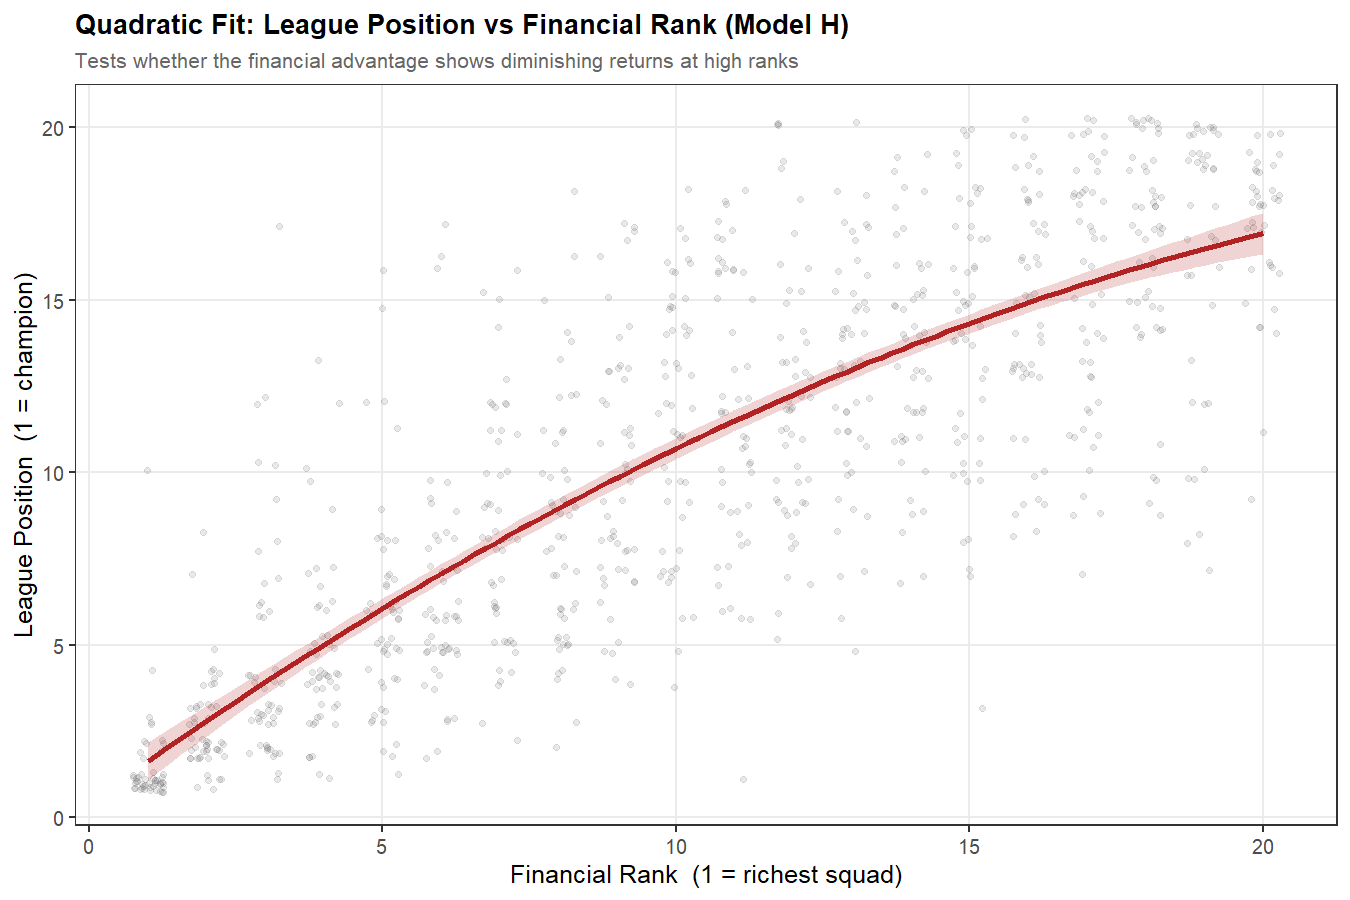
\includegraphics[width=\linewidth,
                       height=0.74\textheight,
                       keepaspectratio]{21_quadratic_fit_plot.png}
    \end{column}
    \begin{column}{0.34\textwidth}
      \vspace{8pt}
      \begin{exampleblock}{What the curve says}
        \vspace{2pt}{\small
        \begin{itemize}
          \setlength\itemsep{6pt}
          \item FR\,1\,$\to$\,2: predicted finish
                moves from \textbf{1.6} to
                \textbf{2.8} ($\Delta = 1.2$ places).
          \item FR\,15\,$\to$\,16: penalty
                shrinks to $\approx 0.6$ places.
          \item The curve flattens at the bottom:
                mid-table spending differences
                matter less.
        \end{itemize}
        }
      \end{exampleblock}
      \vspace{6pt}
      \findingbox{A marginal euro spent by a
        top-2 club buys more league position
        than the same euro spent by a
        mid-table club.}
    \end{column}
  \end{columns}
\end{frame}

\begin{frame}{Champion Probability Drops Sharply With Financial Rank}
  \begin{columns}[T]
    \begin{column}{0.62\textwidth}
      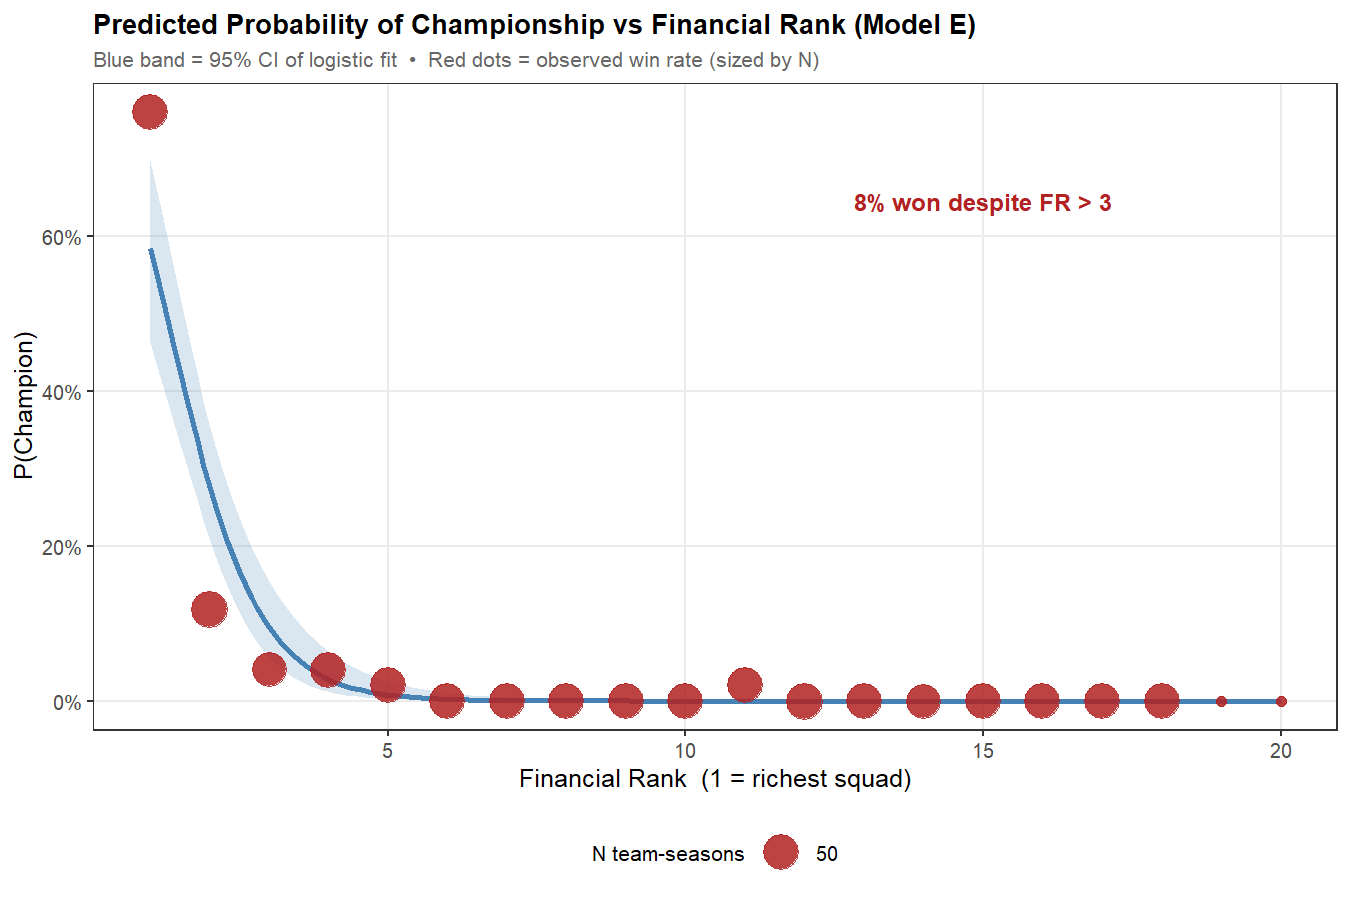
\includegraphics[width=\linewidth,
                       height=0.74\textheight,
                       keepaspectratio]{12_champion_probability_curve.png}
    \end{column}
    \begin{column}{0.34\textwidth}
      \vspace{8pt}
      {\small
      \begin{tabular}{@{}c r@{}}
        \toprule
        \rowcolor{NavyBlue!18}
        \color{white}\textbf{FR} &
        \color{white}\textbf{P(champion)} \\
        \midrule
        1  & 58.5\,\% \\
        \rowcolor{RowA}
        2  & 27.8\,\% \\
        3  &  9.5\,\% \\
        \rowcolor{RowA}
        5  &  0.8\,\% \\
        11 & ${<}0.01$\,\% \\
        \bottomrule
      \end{tabular}
      }
      \vspace{6pt}
      {\footnotesize\color{SlateGrey}
        Logit Model E: Champion\,$\sim$\,FR.
        McFadden $R^2 = 0.55$.
        $\hat{\beta}_{\mathrm{FR}} = -1.30$,
        $p < 0.001$.}
      \vspace{6pt}
      \duallabel{%
        Log-odds fall by $1.30$ per rank step
        (${\approx}73$\,\% odds reduction).}{%
        Winning from outside the richest two
        clubs is statistically almost impossible
        --- but it has happened four times in
        ten years.}
    \end{column}
  \end{columns}
\end{frame}

% ──────────────────────────────────────────────────────────────
%  SECTION 5: The Exceptions
% ──────────────────────────────────────────────────────────────
\section{The Exceptions}

\begin{frame}{76\,\% of Titles Were Won by the League's Richest Club}
  \begin{columns}[T]
    \begin{column}{0.60\textwidth}
      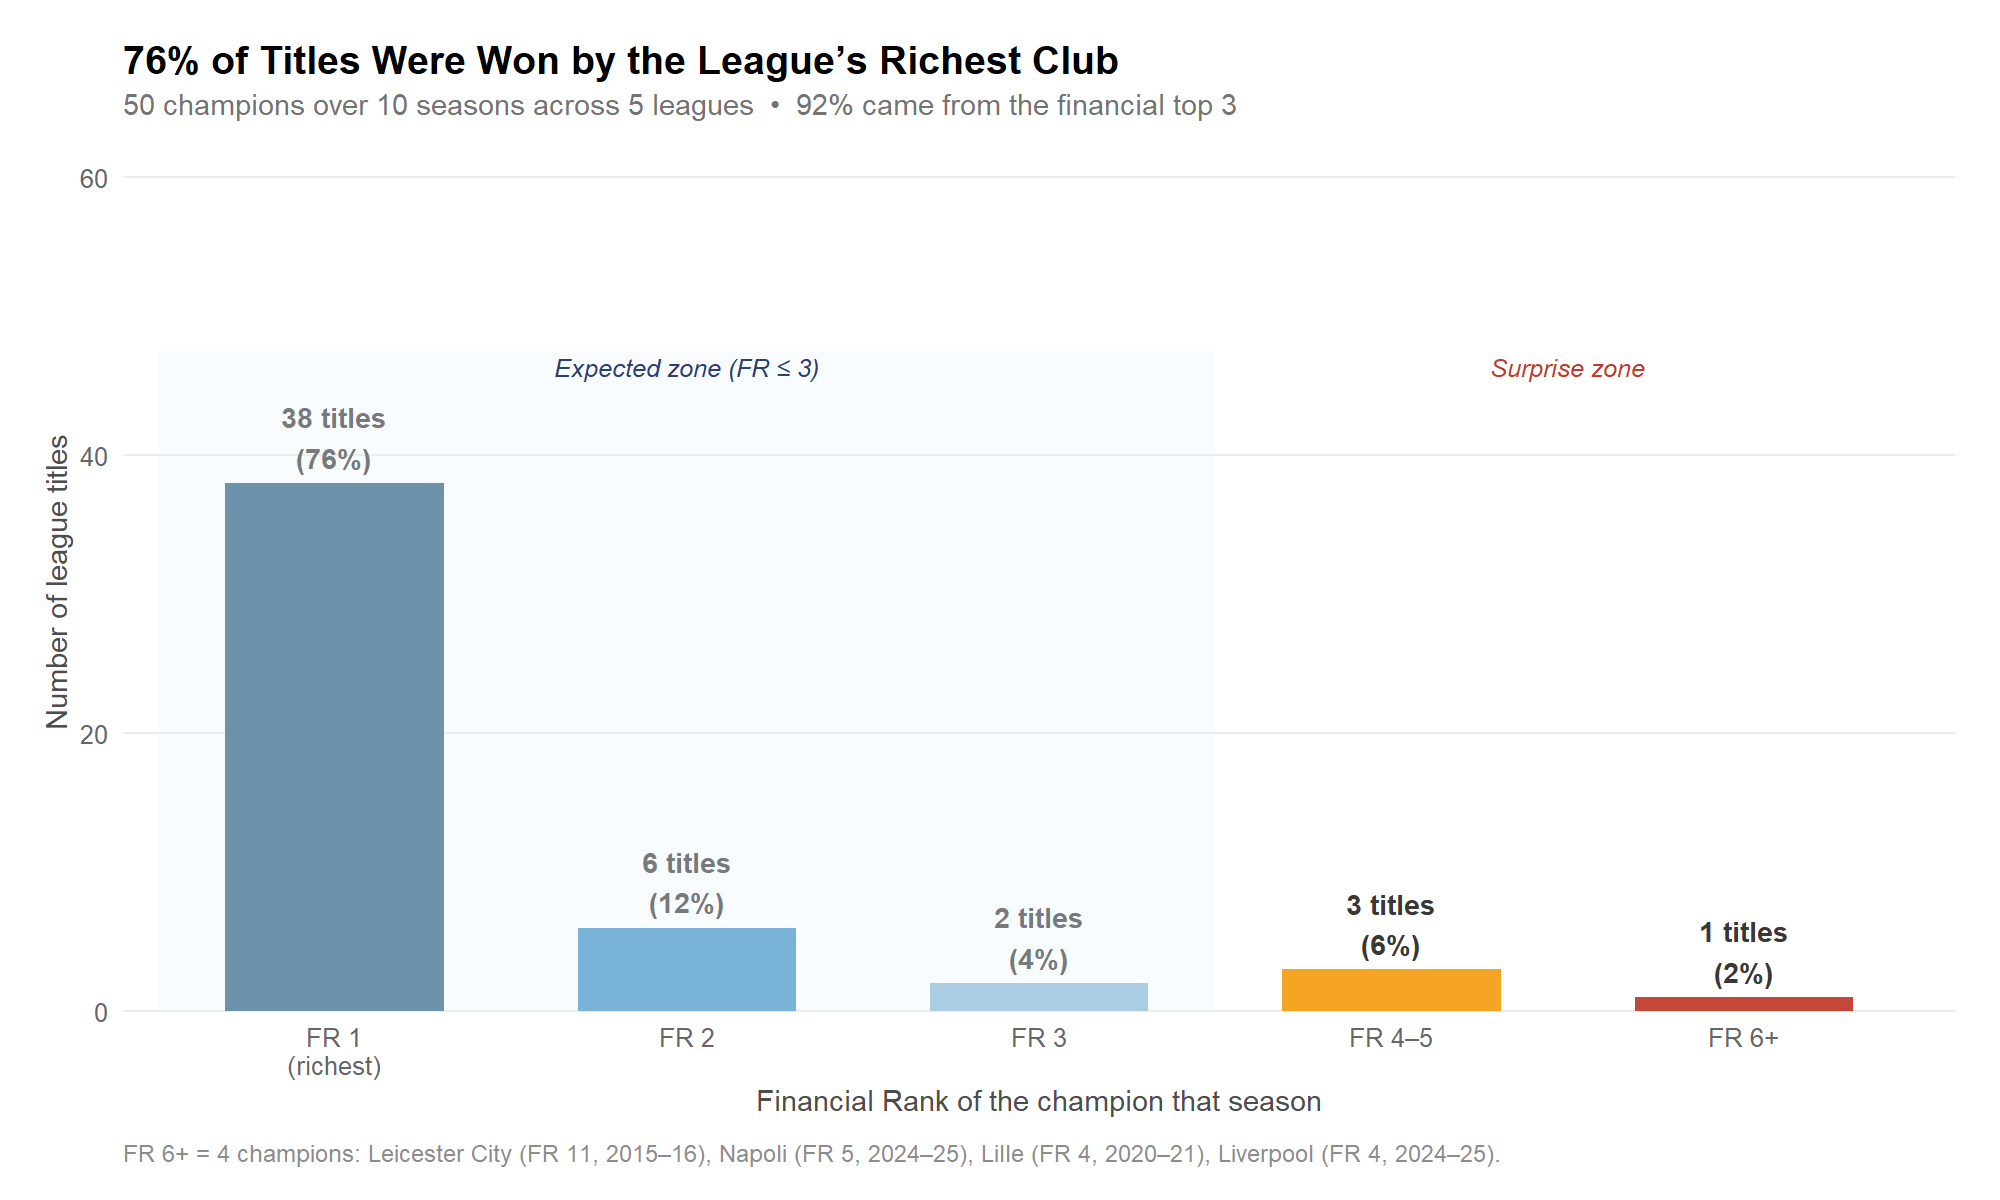
\includegraphics[width=\linewidth,
                       height=0.74\textheight,
                       keepaspectratio]{34_champions_fr_dist.png}
    \end{column}
    \begin{column}{0.36\textwidth}
      \vspace{8pt}
      {\small
      \begin{tabular}{@{}l r r@{}}
        \toprule
        \rowcolor{NavyBlue!18}
        \color{white}\textbf{FR} &
        \color{white}\textbf{Titles} &
        \color{white}\textbf{\%} \\
        \midrule
        1 (richest)       & 38 & 76\,\% \\
        \rowcolor{RowA}
        2                 &  6 & 12\,\% \\
        3                 &  2 &  4\,\% \\
        \rowcolor{RowA}
        4\textendash{}5   &  3 &  6\,\% \\
        \rowcolor{AlertRed!18}
        \textbf{6+}       & \textbf{1} & \textbf{2\,\%} \\
        \midrule
        Total             & 50 & 100\,\% \\
        \bottomrule
      \end{tabular}
      }
      \vspace{6pt}
      \findingbox{92\,\% of champions came from
        the financial top 3. Only 4 clubs (8\,\%)
        won from outside the richest three squads.}
    \end{column}
  \end{columns}
\end{frame}

\begin{frame}{The Four Statistical Upsets \textendash{} Ten Years of Data}
  \vspace{4pt}
  {\small
  \begingroup\setlength{\tabcolsep}{5pt}
  \begin{tabular}{@{}%
    >{\bfseries}p{2.8cm}
    p{2.0cm}
    p{2.7cm}
    c r r@{}}
    \toprule
    \rowcolor{NavyBlue!18}
    \color{white}\textbf{Club} &
    \color{white}\textbf{Season} &
    \color{white}\textbf{League} &
    \color{white}\textbf{FR} &
    \color{white}\textbf{Predicted} &
    \color{white}\textbf{Residual} \\
    \midrule
    \rowcolor{AlertRed!20}
    Leicester City &
      2015\textendash{}16 &
      Premier League &
      \textbf{11} & 11.5 & $\mathbf{-10.5}$ \\
    Napoli &
      2024\textendash{}25 & Serie~A &
      5 & 6.1 & $-5.1$ \\
    \rowcolor{RowA}
    Lille &
      2020\textendash{}21 & Ligue~1 &
      4 & 5.0 & $-4.0$ \\
    Liverpool &
      2024\textendash{}25 &
      Premier League &
      4 & 5.0 & $-4.0$ \\
    \bottomrule
  \end{tabular}
  \endgroup
  }
  \vspace{4pt}
  \begin{columns}[T]
    \begin{column}{0.50\textwidth}
      \alertbox{A \textbf{negative residual} = the club
        finished \textbf{better} than its financial rank
        predicted. Leicester's $-10.5$ positions is the
        largest overperformance in the entire dataset.}
    \end{column}
    \begin{column}{0.46\textwidth}
      \begin{exampleblock}{Also noteworthy}
        \vspace{2pt}{\small
        \textbf{Bayer Leverkusen 2023\textendash{}24}
        (FR = 2): ended Bayern's 11-year Bundesliga
        streak. Residual $= -1.8$
        (within normal range statistically,
        but historically significant).}
      \end{exampleblock}
    \end{column}
  \end{columns}
\end{frame}

\begin{frame}{Leicester City 2015\textendash{}16 \textendash{} A 10-Position Statistical Shock}
  \begin{columns}[T]
    \begin{column}{0.62\textwidth}
      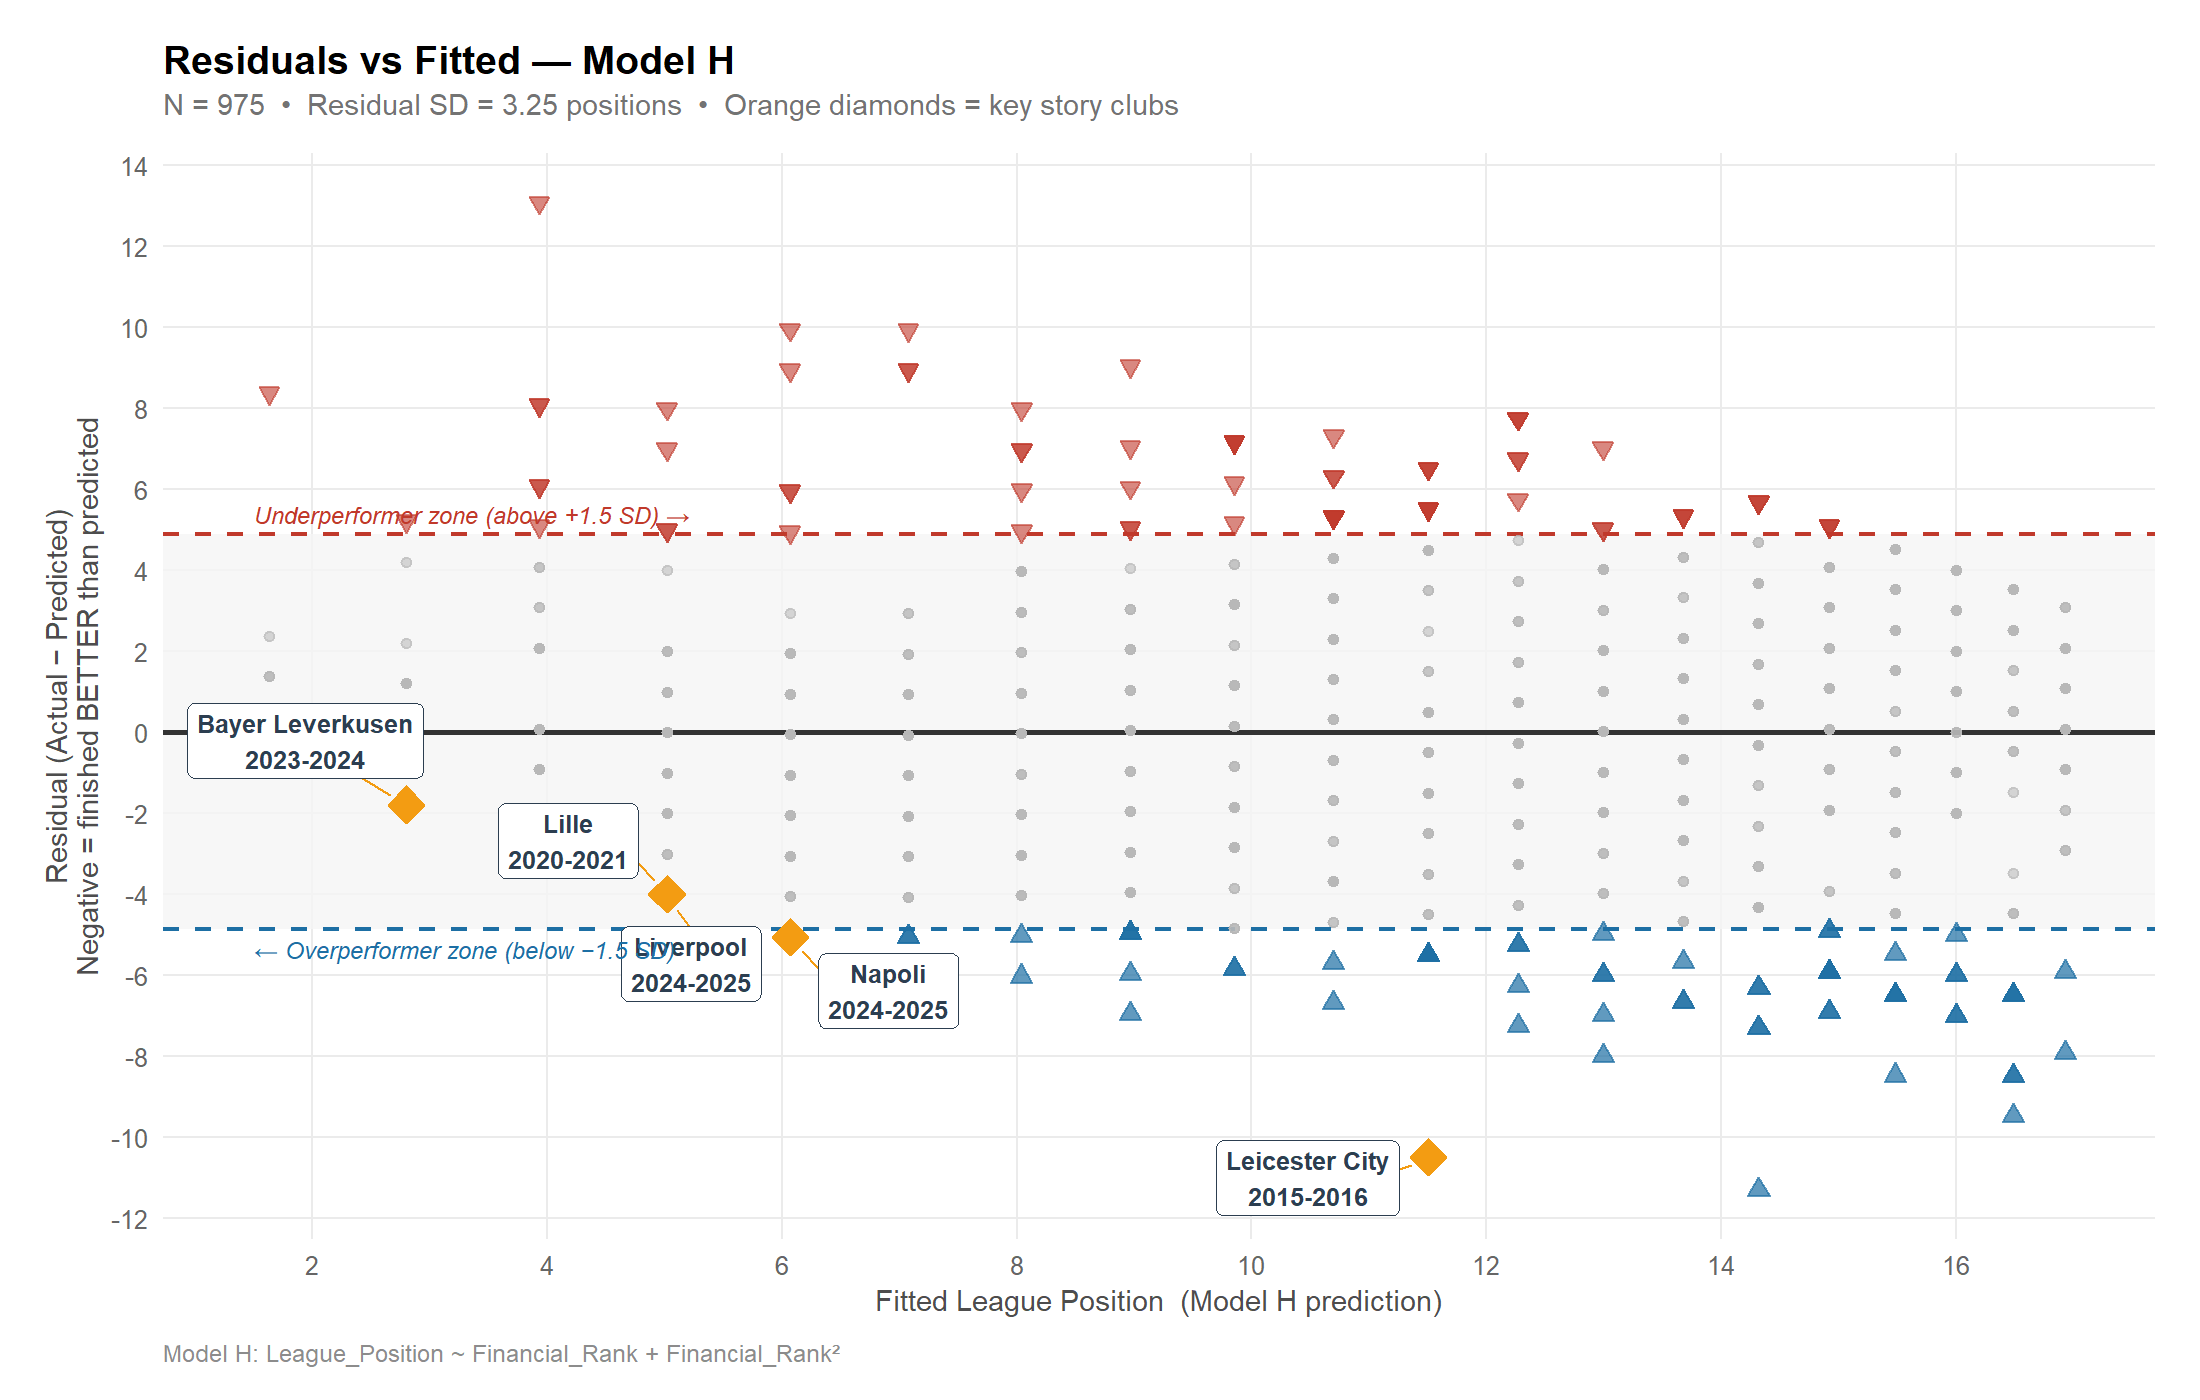
\includegraphics[width=\linewidth,
                       height=0.74\textheight,
                       keepaspectratio]{28b_residual_plot_clean.png}
    \end{column}
    \begin{column}{0.34\textwidth}
      \vspace{8pt}
      \statpanel{Residual $= -10.5$}{Model predicted
        11th place. They finished 1st.}
      \vspace{8pt}
      {\small
      \begin{itemize}
        \setlength\itemsep{6pt}
        \item Only champion to exceed the
              \textbf{$-$1.5\,SD threshold} in
              10 years of data.
        \item FR\,=\,11: squad valued at
              \textsterling{}161\,M vs.\ league
              average \textsterling{}458\,M.
        \item Coach: Claudio Ranieri.
              Bookmaker odds: 5000-to-1.
        \item \alert{Cook's D} = highest in
              the entire dataset, confirming
              genuine statistical leverage.
      \end{itemize}
      }
    \end{column}
  \end{columns}
\end{frame}

\begin{frame}{How the Dotplot Tells the Full Story}
  \begin{columns}[T]
    \begin{column}{0.64\textwidth}
      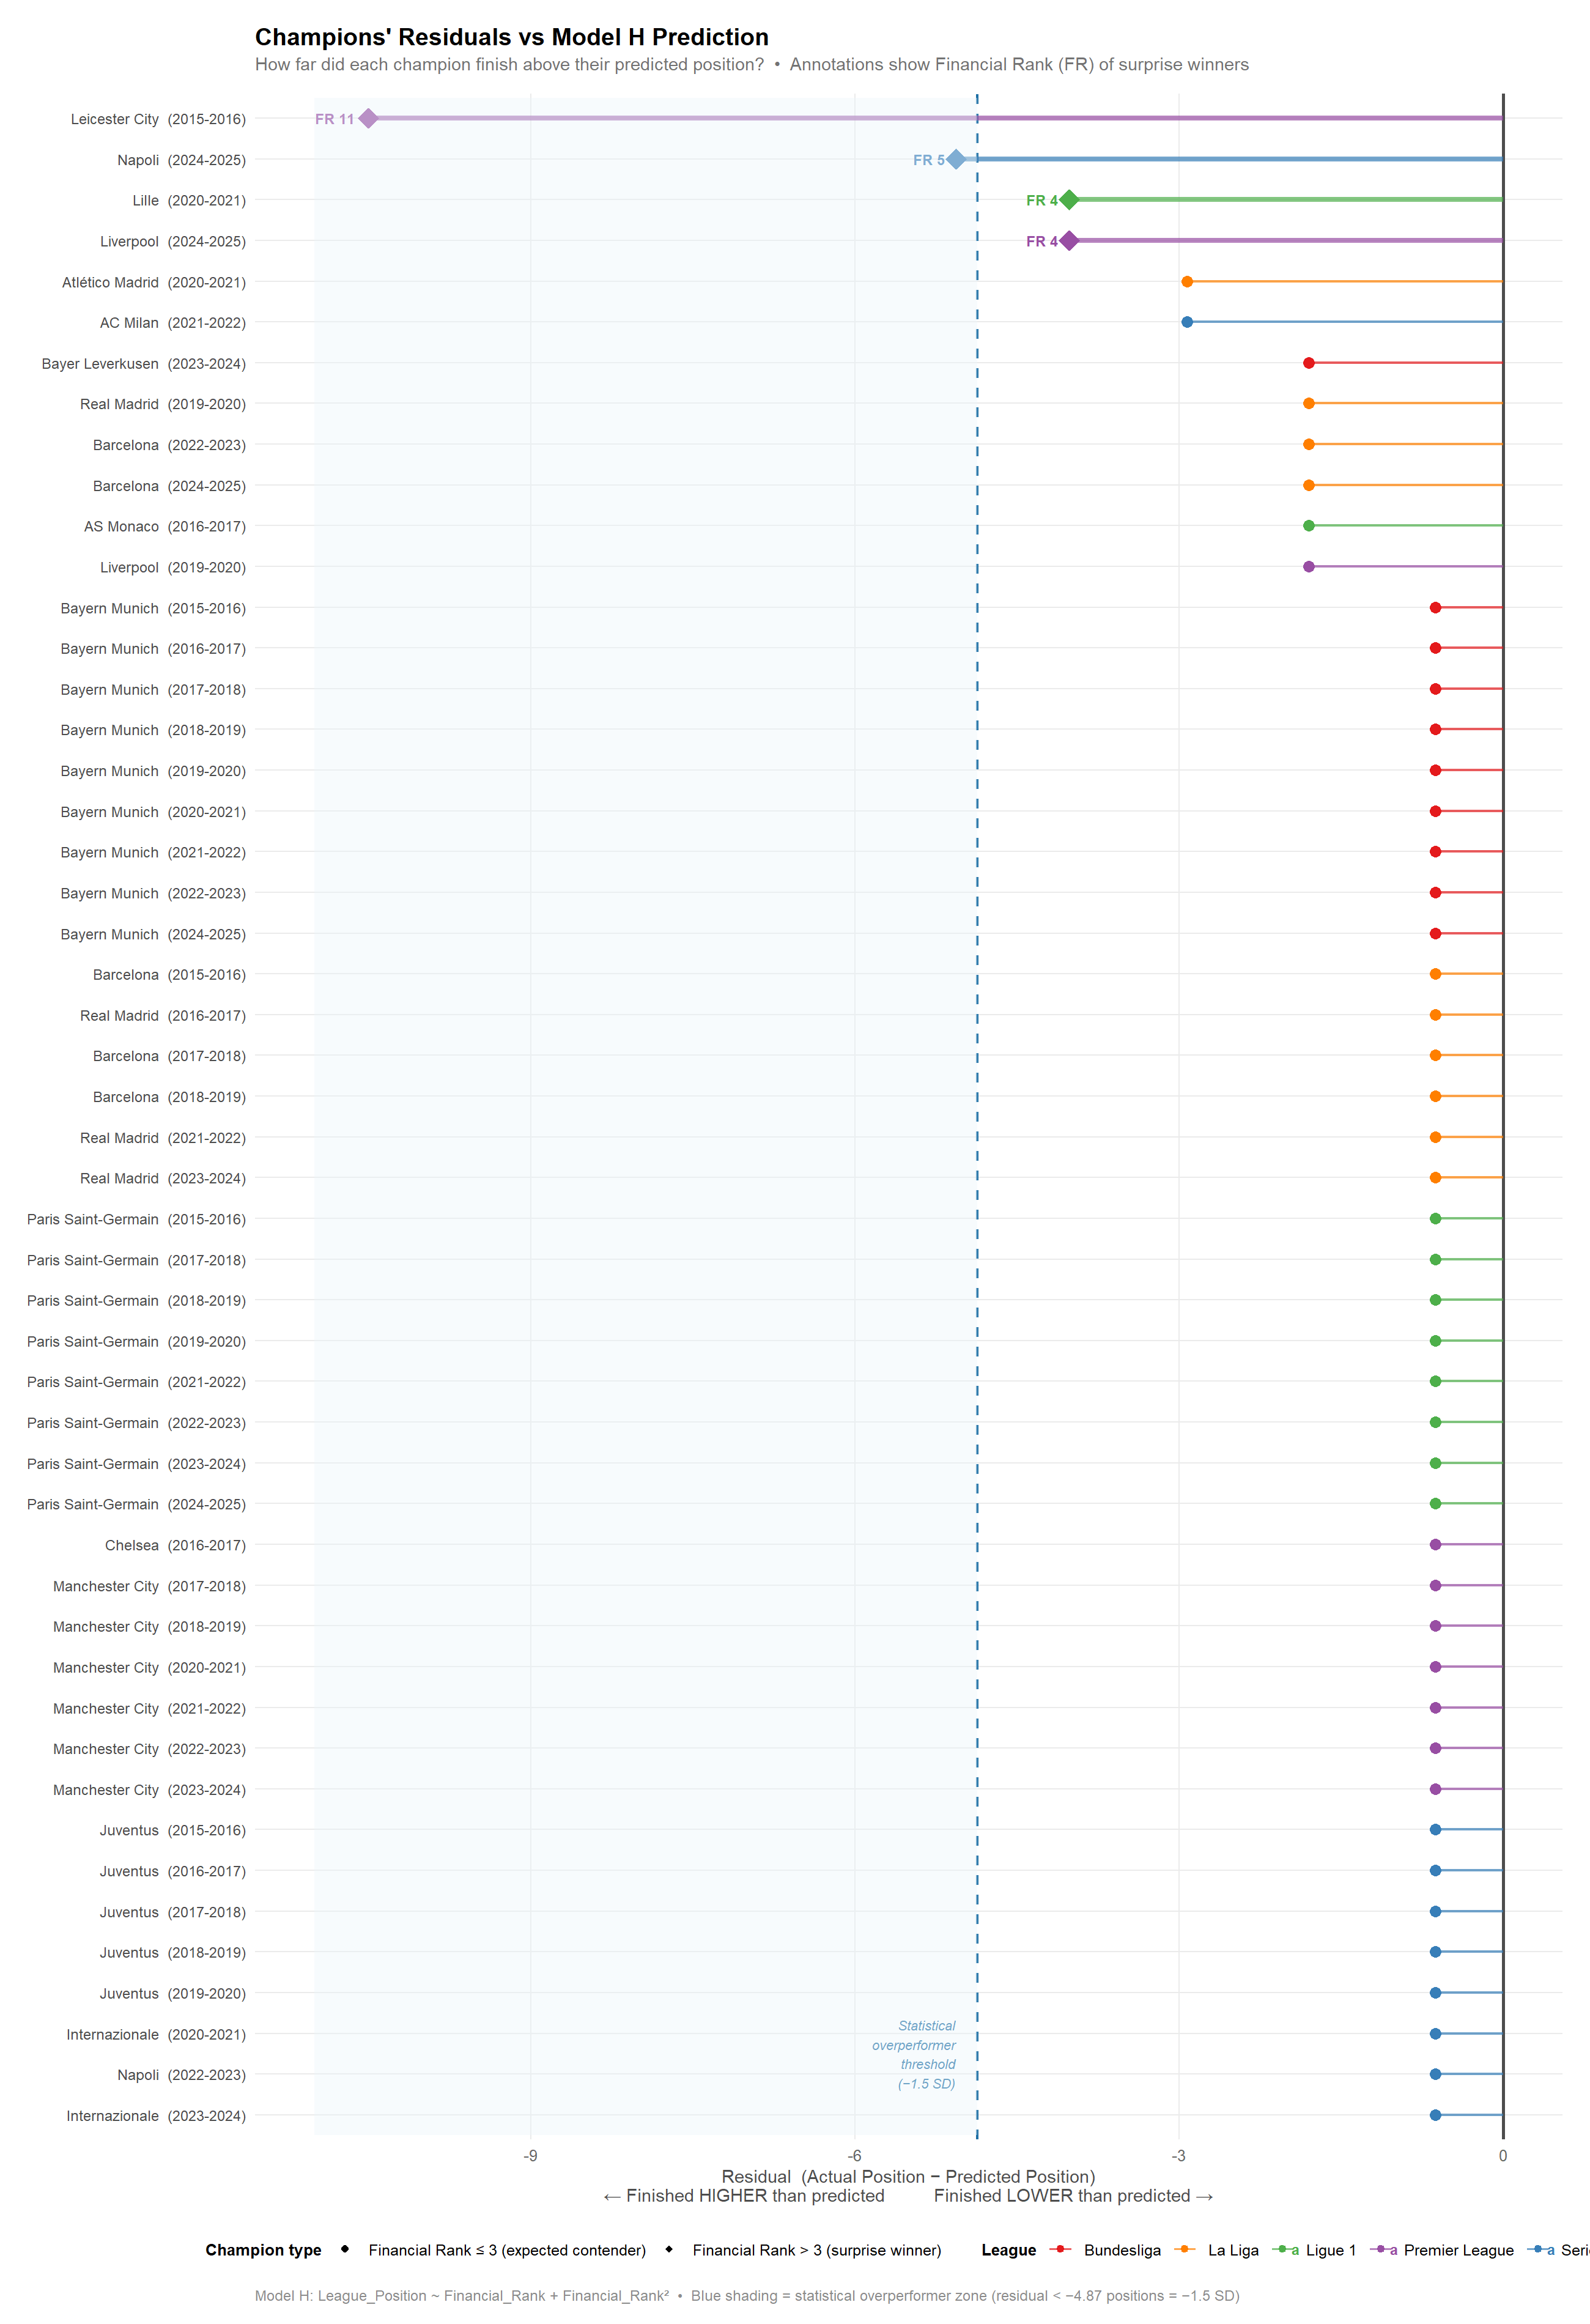
\includegraphics[width=\linewidth,
                       height=0.80\textheight,
                       keepaspectratio]{30b_champions_dotplot_clean.png}
    \end{column}
    \begin{column}{0.32\textwidth}
      \vspace{8pt}
      \begin{block}{Reading the chart}
        \vspace{2pt}{\small
        \begin{itemize}
          \setlength\itemsep{5pt}
          \item Each dot = one league title.
          \item \textbf{Left of zero} = finished
                better than predicted.
          \item \textbf{Diamond} = FR\,$>$\,3
                (surprise winner); label shows FR.
          \item Blue shading = statistical
                overperformer zone
                ($< -1.5$\,SD).
        \end{itemize}
        }
      \end{block}
      \vspace{6pt}
      \findingbox{All 50 champions have
        \textbf{negative} residuals: every title
        winner beat their financial prediction.
        The question is only by \emph{how much}.}
    \end{column}
  \end{columns}
\end{frame}

% ──────────────────────────────────────────────────────────────
%  SECTION 6: Robustness
% ──────────────────────────────────────────────────────────────
\section{Robustness Checks}

\begin{frame}{Three Tests \textendash{} The Core Finding Holds}
  \vspace{4pt}
  {\small
  \begingroup\setlength{\tabcolsep}{4pt}
  \begin{tabular}{@{}%
    p{4.2cm}
    p{3.0cm}
    c
    p{2.8cm}@{}}
    \toprule
    \rowcolor{NavyBlue!18}
    \color{white}\textbf{Test} &
    \color{white}\textbf{Statistic} &
    \color{white}\textbf{$p$-value} &
    \color{white}\textbf{Verdict} \\
    \midrule
    Quadratic vs.\ linear &
      $F = 31.7$ (1\,df) &
      $<0.001$ &
      \textcolor{GrassGreen}{\textbf{Quadratic confirmed}} \\
    \rowcolor{RowA}
    League interaction (FR\,$\times$\,League) &
      $F = 1.17$ (4\,df) &
      $0.32$ &
      \textcolor{SlateGrey}{Effect uniform} \\
    Time trend (FR\,$\times$\,Season) &
      $F = 0.44$ (1\,df) &
      $0.51$ &
      \textcolor{SlateGrey}{Stable 2015\textendash{}25} \\
    \rowcolor{RowA}
    Heteroskedasticity &
      BP $\chi^2 = 45.5$ &
      $<0.001$ &
      \textcolor{AlertRed}{Present; HC1 SEs used} \\
    \midrule
    \rowcolor{RowB}
    \multicolumn{2}{@{}l}{\textbf{FR coeff.\ under HC1 robust SEs}} &
      $<0.001$ &
      \textcolor{GrassGreen}{\textbf{Robust}} \\
    \bottomrule
  \end{tabular}
  \endgroup
  }
  \vspace{4pt}
  \begin{columns}[T]
    \begin{column}{0.48\textwidth}
      \findingbox{The FR effect is statistically
        identical across all five leagues and has
        not strengthened or weakened over the
        ten seasons studied.}
    \end{column}
    \begin{column}{0.48\textwidth}
      \duallabel{%
        Breusch\textendash{}Pagan $\chi^2=45.5$,
        $p<0.001$; corrected with HC1
        heteroskedasticity-robust SEs.}{%
        Prediction errors vary in size across
        the position range, so we use corrected
        standard errors to ensure valid inference.}
    \end{column}
  \end{columns}
\end{frame}

% ──────────────────────────────────────────────────────────────
%  SECTION 7: Conclusions
% ──────────────────────────────────────────────────────────────
\section{Conclusions}

\begin{frame}{Key Findings \textendash{} Three Takeaways}
  \begin{columns}[T]
    \begin{column}{0.55\textwidth}
      \vspace{4pt}
      \begin{enumerate}
        \setlength\itemsep{10pt}
        \item \textbf{Money predicts position strongly.}\\
              {\small Financial Rank alone explains
              \textbf{67\,\%} of variation in final
              standing (Model H, $R^2 = 0.671$;
              $r = 0.813$ across 975 observations).}

        \item \textbf{Surprises are statistically rare.}\\
              {\small Only 4 of 50 champions (8\,\%)
              came from outside the richest three
              squads. Leicester City 2015\textendash{}16
              is the lone statistical outlier
              (residual $= -10.5$ positions).}

        \item \textbf{The effect is stable and non-linear.}\\
              {\small The quadratic term ($p < 0.001$)
              shows diminishing returns at the bottom;
              the time-trend interaction is not
              significant ($p = 0.51$).}
      \end{enumerate}
    \end{column}
    \begin{column}{0.41\textwidth}
      \vspace{4pt}
      \findingbox{For statisticians: Model H
        ($\hat{\beta}_{\mathrm{FR}} = 1.23$,
        $\hat{\beta}_{\mathrm{FR}^2} = -0.020$,
        AIC = 5070.5) outperforms all tested
        specifications.}
      \vspace{8pt}
      \findingbox{For fans: being the richest club
        gives a 58\,\% championship probability.
        Being the 5th-richest drops that to under
        1\,\%. Football still surprises us --- just
        not very often.}
      \vspace{8pt}
      \begin{exampleblock}{Limitations}
        {\small\begin{itemize}
          \setlength\itemsep{3pt}
          \item Market value as proxy for quality
                (injuries, form ignored).
          \item Managerial quality not modelled.
          \item Five leagues may not generalise
                to lower divisions.
        \end{itemize}}
      \end{exampleblock}
    \end{column}
  \end{columns}
\end{frame}

\begin{frame}{Thank You \textendash{} Questions?}
  \begin{columns}[T]
    \begin{column}{0.54\textwidth}
      \vspace{8pt}
      {\large\bfseries\color{NavyBlue}
       Money and Success in Football}\\[4pt]
      {\color{SlateGrey}\small
       Does Financial Strength Predict League Position?}
      \vspace{12pt}

      \statpanel{$r=0.813$\quad $R^2=0.671$\quad $N=975$}{%
        Five leagues\,$\cdot$\,ten seasons\,$\cdot$\,one answer:
        \textbf{yes, mostly}}

      \vspace{10pt}
      {\small\color{SlateGrey}
      \textbf{Data:} ESPN Standings + Transfermarkt\\
      \textbf{Period:} 2015\textendash{}16 to
        2024\textendash{}25\\
      \textbf{Models:} OLS (A\textendash{}H), Logit
        (E, F, J), Ordinal Logit (K)\\
      \textbf{Contact:}
        \url{mdmuktadir0611@gmail.com}}
    \end{column}
    \begin{column}{0.42\textwidth}
      \vspace{8pt}
      \begin{block}{Appendix / Backup Slides Available}
        {\small
        \begin{itemize}
          \setlength\itemsep{5pt}
          \item Full model coefficient table
                (Models A\textendash{}H)
          \item Cook's distance diagnostics
          \item Ordinal logistic results (Model K)
          \item Season-by-season champion FR table
          \item League interaction slopes (Model G)
        \end{itemize}
        }
      \end{block}
      \vspace{6pt}
      \alertbox{The one exception everyone
        remembers: Leicester City 2015\textendash{}16.
        FR\,=\,11. Residual\,$= -10.5$\,positions.
        The model said 11th. They won the league.}
    \end{column}
  \end{columns}
\end{frame}

% ──────────────────────────────────────────────────────────────
%  APPENDIX
% ──────────────────────────────────────────────────────────────
\appendix

\begin{frame}{Appendix A \textendash{} Full Model Comparison}
  \vspace{2pt}
  {\footnotesize
  \begingroup\setlength{\tabcolsep}{4pt}
  \begin{tabular}{@{}%
    >{\bfseries}c
    p{4.2cm}
    r r r r@{}}
    \toprule
    \rowcolor{NavyBlue!18}
    \color{white}\textbf{Mdl} &
    \color{white}\textbf{Formula} &
    \color{white}\textbf{$R^2$} &
    \color{white}\textbf{Adj.$R^2$} &
    \color{white}\textbf{AIC} &
    \color{white}\textbf{$N$} \\
    \midrule
    A & FR             & 0.660 & 0.660 & 5099.8 & 975 \\
    \rowcolor{RowA}
    B & FR + League    & 0.660 & 0.659 & 5107.4 & 975 \\
    C & Log(MV)        & 0.533 & 0.532 & 5410.6 & 975 \\
    \rowcolor{RowA}
    D & Log(MV) + League + Season & 0.641 & 0.639 & 5164.3 & 975 \\
    G & FR $\times$ League  & 0.651 & 0.645 & 5110.7 & 975 \\
    \rowcolor{RowB}
    \textbf{H} &
    \textbf{FR} $+$ \textbf{FR}$^2$ &
    \textbf{0.671} & \textbf{0.670} &
    \textbf{5070.5} & \textbf{975} \\
    I & FR $\times$ Season & 0.651 & 0.649 & 5103.4 & 975 \\
    \midrule
    E & Champion $\sim$ FR (Logit) &
      \multicolumn{2}{c}{McFadden\,=\,0.548} & 182.4 & 975 \\
    \rowcolor{RowA}
    F & Champion $\sim$ Log(MV)+League (Logit) &
      \multicolumn{2}{c}{McFadden\,=\,0.592} & 173.1 & 975 \\
    \bottomrule
  \end{tabular}
  \endgroup
  }
  \vspace{4pt}
  {\footnotesize\color{SlateGrey}
   OLS response: League\_Position (1\,=\,champion).
   Bold\,=\,best OLS by AIC. Model~F\,=\,best logistic.}
\end{frame}

\begin{frame}{Appendix B \textendash{} Cook's Distance Diagnostics}
  \begin{columns}[T]
    \begin{column}{0.64\textwidth}
      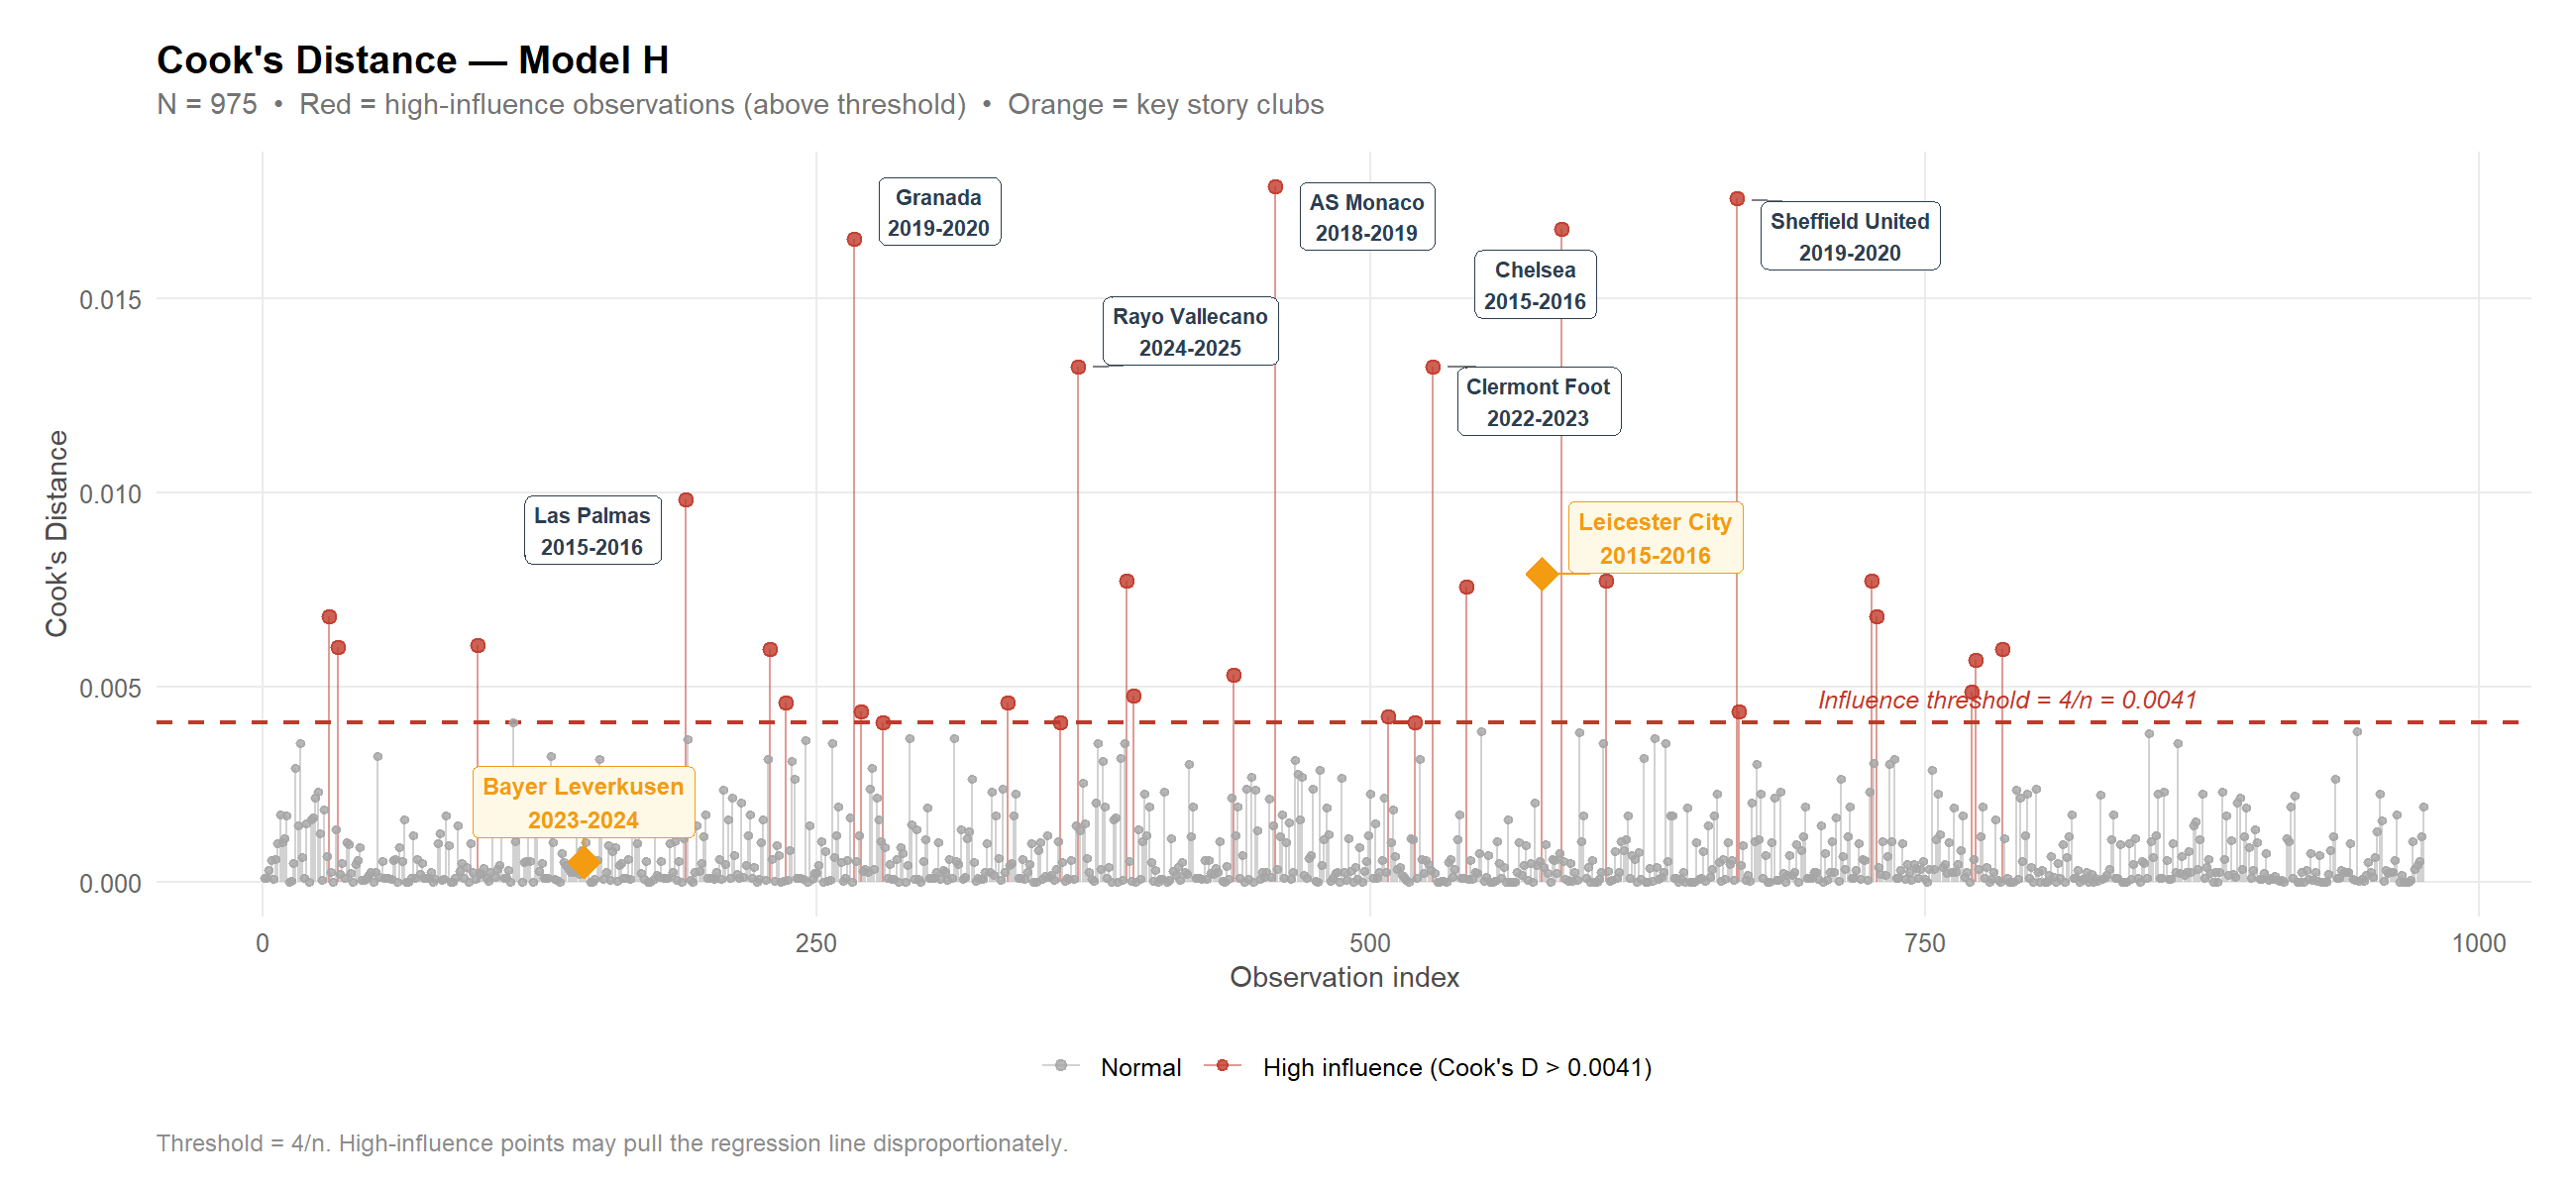
\includegraphics[width=\linewidth,
                       height=0.74\textheight,
                       keepaspectratio]{29b_cooks_distance_clean.png}
    \end{column}
    \begin{column}{0.32\textwidth}
      \vspace{8pt}
      \begin{block}{Interpreting Cook's D}
        {\small
        \begin{itemize}
          \setlength\itemsep{5pt}
          \item Threshold $= 4/n = 0.0041$.
          \item High-influence points can
                pull the regression line
                disproportionately.
          \item Leicester City is both the
                \textbf{largest residual} and
                the \textbf{highest Cook's D}.
          \item Removing Leicester raises the
                intercept slightly but does not
                change slope direction.
        \end{itemize}
        }
      \end{block}
      \vspace{6pt}
      \duallabel{%
        Leicester's Cook's D well above threshold;
        it is the dominant leverage point in
        the dataset.}{%
        Leicester is a genuine outlier, not a
        data error. Removing it makes the
        FR\textendash{}position relationship
        \emph{stronger}, not weaker.}
    \end{column}
  \end{columns}
\end{frame}

\begin{frame}{Appendix C \textendash{} Interaction Slopes by League (Model G)}
  \begin{columns}[T]
    \begin{column}{0.62\textwidth}
      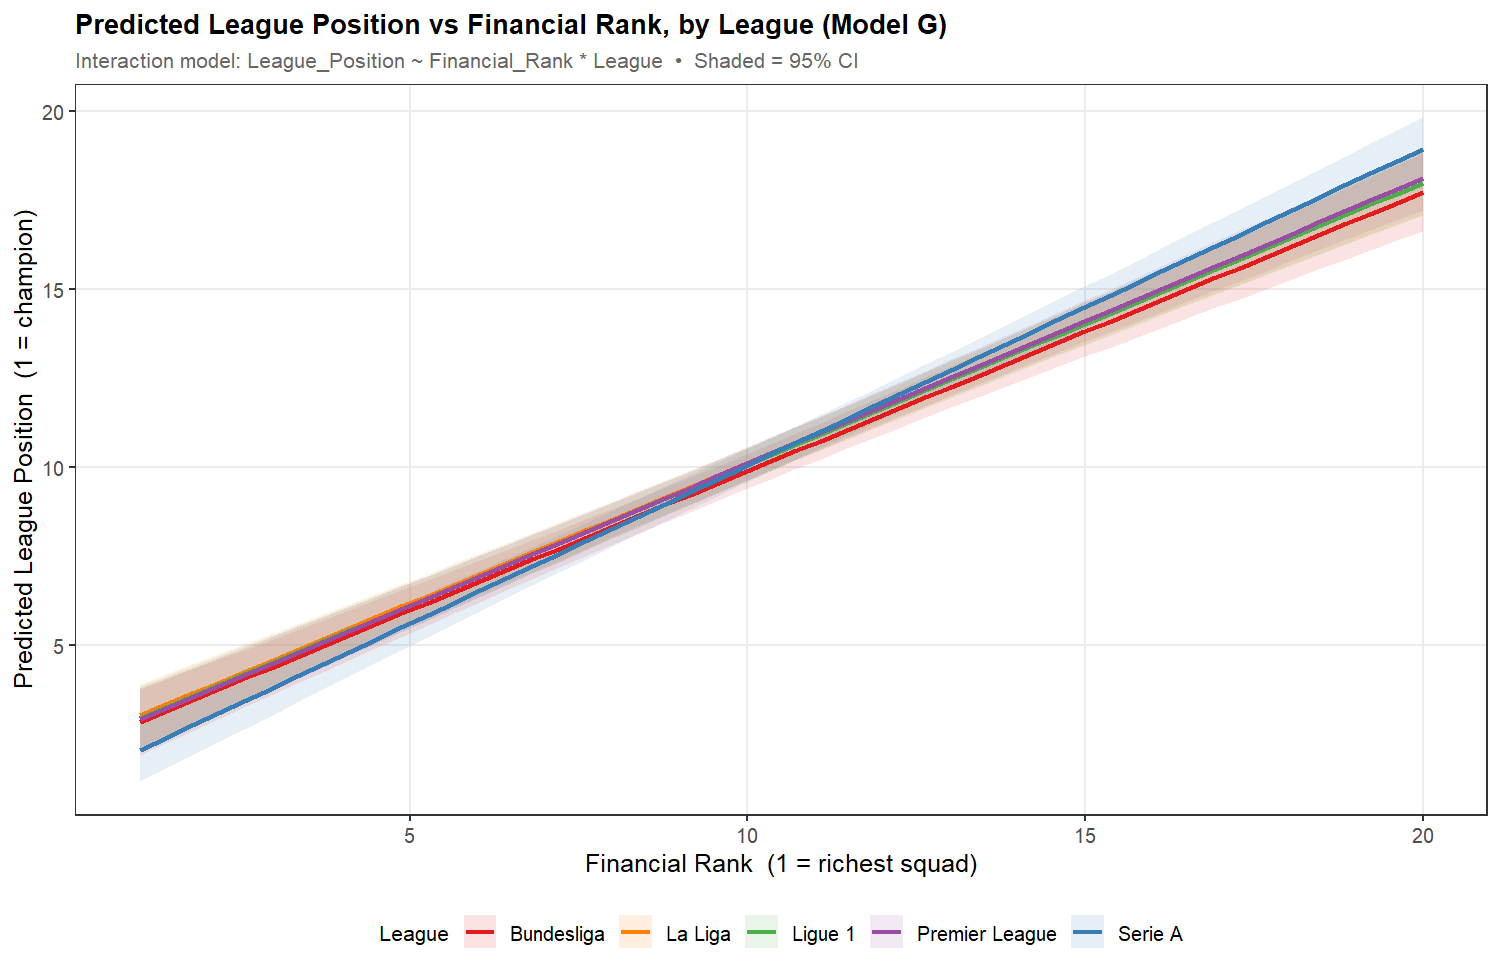
\includegraphics[width=\linewidth,
                       height=0.74\textheight,
                       keepaspectratio]{19_interaction_slopes_by_league.png}
    \end{column}
    \begin{column}{0.34\textwidth}
      \vspace{8pt}
      \begin{block}{Model G: FR $\times$ League}
        {\small
        \begin{itemize}
          \setlength\itemsep{6pt}
          \item Interaction $F = 1.17$,
                $p = 0.32$ $\Rightarrow$
                \textbf{not significant}.
          \item Slopes are visually parallel:
                the financial advantage is the
                same size in all five leagues.
          \item Serie~A slope slightly steeper,
                consistent with its highest $R^2$.
        \end{itemize}
        }
      \end{block}
      \vspace{6pt}
      \findingbox{Money works the same way in
        Munich, Madrid, Milan, Marseille, and
        Manchester. The mechanism is
        league-invariant.}
    \end{column}
  \end{columns}
\end{frame}

\end{document}
